\documentclass[t,presentation,10pt,xcolor=table]{beamer}
\usetheme{Antibes}
\usecolortheme{lily}
\usefonttheme[onlymath]{serif}
\usepackage{xfrac}
\usepackage{adjustbox}
\title[Allele frequencies in autopolyploids]{Estimating allele frequencies in non-model [auto]polyploids using high throughput sequencing data}
\author[Botany 2015]{Paul Blischak$^1$, Laura Kubatko$^{1,2}$, Andrea Wolfe$^1$}
\institute[Edmonton]
{\bfseries
$^1$Dept. of EEOB \\
$^2$Dept. of Statistics \\
The Ohio State University
}
\date{\today}

\begin{document}

\frame{\titlepage}

\begin{frame}
\frametitle{Outline}
\tableofcontents
\end{frame}

\section{Historical background}
\subsection{Early empiricists}

\begin{frame}
\frametitle{Early empiricists}

\end{frame}

\begin{frame}[plain]{}
	\begin{center}
		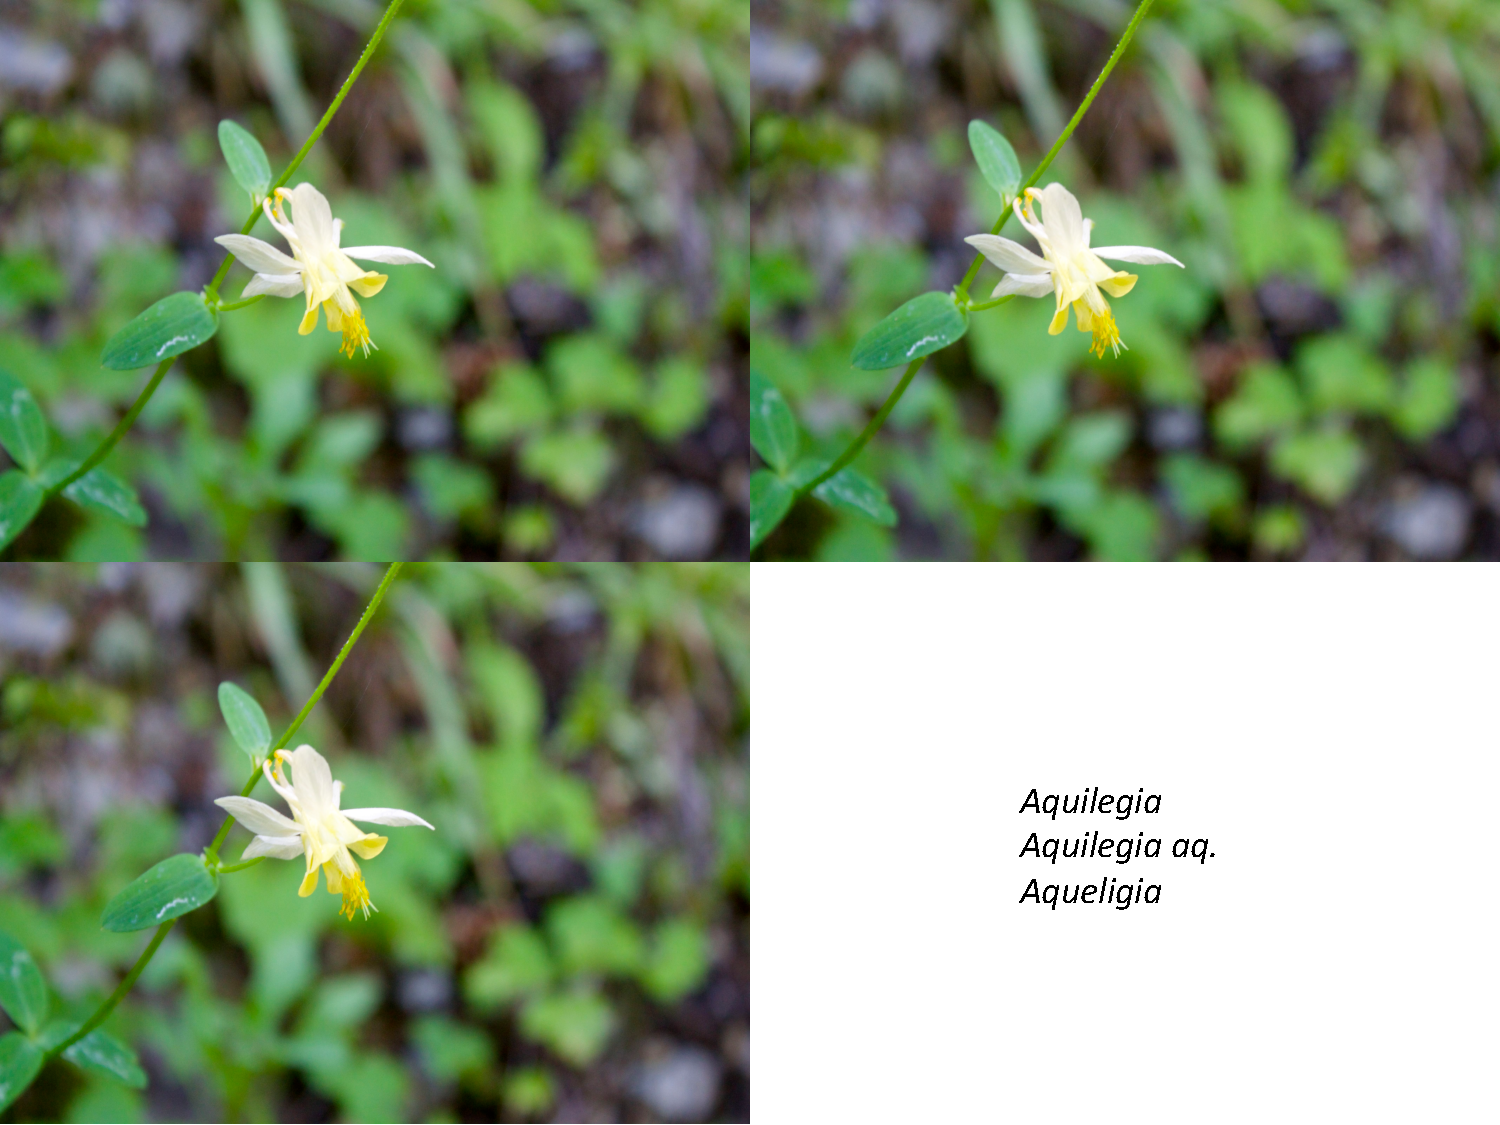
\includegraphics[width=\textwidth]{figs/test}
	\end{center}
\end{frame}

\subsection{Early theory}

\begin{frame}
\frametitle{Early theory}
\begin{itemize}
	\item \textbf{Haldane} -- Models for autopolyploids.
	\item \textbf{Fisher} -- Models for autopolyploids inheritance w/ double reduction.
	\item \textbf{Wright} -- Models for the distribution of allele frequencies in autopolyploids.
\end{itemize}

\end{frame}

%

\section{Population genetics models}


\end{document}